\documentclass[11pt]{article}
\usepackage{graphicx}
\usepackage{hyperref}
\usepackage{caption}
\usepackage{amsmath}
\usepackage{amssymb}
\usepackage{color}
\usepackage{mathtools}
\usepackage{physics}
\usepackage{listings}
\usepackage{xcolor}
\usepackage{subfig}
\newcommand{\numpy}{{\tt numpy}}    % tt font for numpy

\topmargin -.5in
\textheight 9in
\oddsidemargin -.25in
\evensidemargin -.25in
\textwidth 7in

\graphicspath{ {./imgs/}
               {../} }

\usepackage{dirtree}

\begin{document}

% ========== Edit your name here
\author{Jongwon Lee (NetID: 670848047)}
\title{CS 498: Assignment 5: 3D Multi Object Tracking}
\date{\today}
\maketitle

\medskip


\section*{Submission}

You will be submitting two files, "kalman\_filter.py" and "matching.py". Please put together a single PDF with your answers and figures for each problem, and submit it to Gradescope (Course Code: JBXJVZ). 
We recommend you add your answers to the latex template files we provided. More details on what to report are in the provided code. 

Reminder: please put your name and netid in your pdf.

\section*{Provided Files}

\textbf{Files you will modify}:
\begin{itemize}
    \item kalman\_filter.py: 
    \begin{itemize}
        \item define\_model (define dynamics)
        \item update (observation model)
        \item predict (state propagation)
    \end{itemize}
    \item matching.py (greedy matching algorithm)
    \item main.py (for visualization and debugging)
\end{itemize}

\noindent \textbf{Files you will not (need to) modify}:
\begin{itemize}
    \item evaluate.py: run this after running main.py to do evaluation, i.e. "python evaluate.py"
    \item kitti\_calib/oxts.py: these are used for something called ego-motion-compensation, explained in code
    \item matching\_utils.py: contains the function iou(box\_a, box\_b) which you will need to compute similarity when doing matching
    \item utils.py: some utils used by main.py, you should look at Box3D
    \item vis.py: some code for visualizing the data. You only really need vis\_obj, which is described more clearly in main.py
\end{itemize}

File structure
\dirtree{%
.1 data.
.2 calib.
.3 training.
.4 [seq\_name].txt.
.2 detection.
.3 [seq\_name].txt.
.2 label.
.3 [seq\_name].txt.
.2 oxts.
.3 training.
.4 [seq\_name].txt.
.2 image\_02.
.3 training.
.4 [seq\_name].
.5 [frame\_num].png.
.1 results.
.2 eval (files in here will be created automatically).
.2 img\_vis (files in here will be created automatically).
}

\section*{Multi Object Tracking (MOT)} 

In this assignment, you will implement a multi object tracker for 3D objects. In other words, given a sequence of frames taken from the perspective of a car, track the other cars in the images. In this project we will develop our tracking algorithm on KITTI dataset(\url{http://www.cvlibs.net/datasets/kitti/}). 

The idea is as follows: we can use a good pre-trained object detector to find objects in each frame (we've already done that for you, check \url{https://github.com/sshaoshuai/PointRCNN} if you want to know more). Now, simply identifying objects is not good enough, so we want to track them across frames for consistency. You will implement two main methods which together will do this quite well. 

The first is a matching algorithm: given a list of 3D bounding boxes for objects detected by the object detector in the current frame, match them to objects you are already tracking from the previous frame. 

The second is a Kalman Filter. Just matching current detections to past trackers is not great since cars can move and therefore the previous and current bounding boxes will not overlap perfectly (this is especially problematic if an object becomes occluded for a few frames). To deal with this issue you will implement a Kalman Filter for forward propagating each object. Moreover, you will now use each object detection to "update" the state of your tracked object, as an observation to the filter.

% DONE
\paragraph{Question 0 (Inspect the Data)[1 pt]:}
Before you begin the actual assignment, read the code we've provided. Namely read through "main.py" so you understand the basic structure of the algorithm and the functionality of each component. You will need to modify main.py, but only for debugging/visualization purposes. 

For this question, please visualize the detections for frame 100 of the first and second sequences, i.e. sequence 0000 and sequence 0001. Each detection should be a different color. You should work off the code we provided in the Visualization section of main.py.

Please download the images for the first sequence (0000), and put them in the right place in the directory structure above. Use your illinois address to access the drive link: \url{https://drive.google.com/file/d/15lWATvV4p9UCShnnPa2SEL8BTh2twIm4/view?usp=sharing}
\paragraph{Answer:} 
\begin{quote}

Below is the code for plotting object detections on the image, without any bayesian filtering methods:

\begin{lstlisting}[language=Python, basicstyle=\scriptsize]

matched, unmatched_dets, unmatched_trks = data_association(frame_dets, trks_bbox, 
                                                           threshold=-0.2, algm=algm)

if is_Q0:
    for det in frame_dets:
        trk_color = tuple([int(tmp * 255) for tmp in cmap[i % 256][:3]])
        img = vis_obj(det, img, calib, hw, trk_color)

\end{lstlisting}

Visualizations of the detections for frame 100 of the first and second sequences, i.e. sequence 0000 and sequence 0001., are in Fig.~\ref{fig:q0}.

% detected objects at 100th frame in sequence 0000 and sequence 0001
\begin{figure}[h]
    \centering
    \subfloat {{ 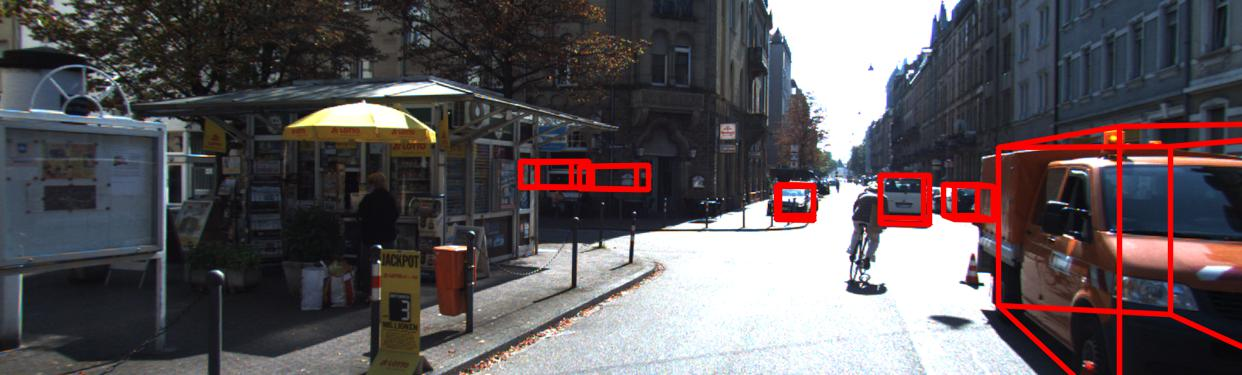
\includegraphics[width=0.9\linewidth]{Q0_0000_100.jpg} }} \\
    \subfloat {{ 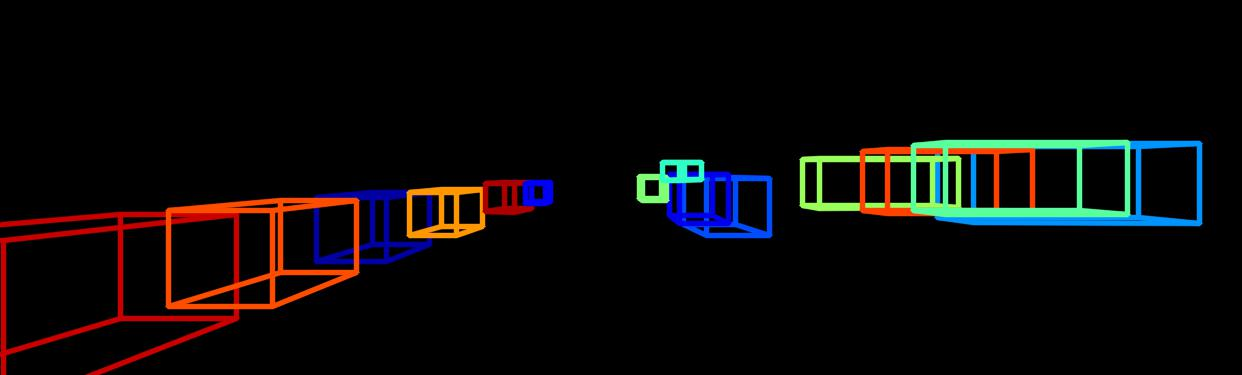
\includegraphics[width=0.9\linewidth]{Q0_0001_100.jpg} }}
    \caption{Detections for the frame 100 of the sequence 0000 (top) and 0001 (below).}
    \label{fig:q0}
\end{figure}

\end{quote}

% DONE
\paragraph{Question 1 (Greedy Matching)[3 pt]:}
For this question you will be modifying "matching.py". You should implement a greedy matching approach, whereby you match pairs of detections and tracked objects in order of similarity. First match the detection and tracker that are most similar, then remove them from the set, and continue, until you have no trackers or no detections. Also, if the similarity for a match is more than the provided threshold, do not consider the pair a match.

Notice we provide you with "iou(box\_a, box\_b)" to compute similarity between 3D detected regions.
\paragraph{Answer:} 
\begin{quote}

Below is the code for performing greedy matching between the tracked objects (from the past frames) and detections (at the current frame), following the instruction as described:

\begin{lstlisting}[language=Python, basicstyle=\scriptsize]

# Begin with sets of unmatched_dets and unmatched_trks
unmatched_dets = list(range(len(dets)))
unmatched_trks = list(range(len(trks)))

# Continue until either unmatched_dets or unmatched_trks become empty
while (len(unmatched_dets) is not 0) and (len(unmatched_trks) is not 0):
    # Find best matching pair between dets and trks
    iou_max = -np.inf
    det_i_max = None
    trk_i_max = None
    for det_i in unmatched_dets:
        for trk_i in unmatched_trks:
            iou_max = max(iou_max, iou(dets[det_i], trks[trk_i]))
            if iou_max == iou(dets[det_i], trks[trk_i]):
                det_i_max = det_i
                trk_i_max = trk_i
    
    if (iou_max < threshold) or (iou_max == -np.inf):
        # If the found iou_max is smaller than threshold, stop
        break
    else:
        # Otherwise, add the pair to matches, 
        # remove them from unmatched sets, and continue
        matches.append((det_i_max, trk_i_max))
        unmatched_dets.remove(det_i_max)
        unmatched_trks.remove(trk_i_max)

\end{lstlisting}

\end{quote}

% DONE
\paragraph{Question 2 (Trivial Update) [1 pt]:}
You'll notice that even though you've implemented matching, the trackers themselves don't update location. For this question you will implement a trivial update to each tracker in kalman\_filter.py. Given a matched detection z, simply set the associated tracker to have the same bounding box z. In other words, we simply trust the observation 100\% when updating the state, neglecting any motion or noise models.

In your pdf please show your code for this part, it should be very simple. Report your evaluation MOTA for this setting (meaning matching=greedy, predict() is unimplemented, and the update is trivial).
\paragraph{Answer:} 
\begin{quote}

Below is the code for trivial update (i.e., trust an object detection result as it is):

\begin{lstlisting}[language=Python, basicstyle=\scriptsize]

def update(self, z, kalman_update=False):
    ...

    if kalman_update:  # For Q4 and Q5
        ...
    else:              # For Q2
        # Trust measurement (detection) as it is
        self.x[:7] = z

    ...

\end{lstlisting}

Note that any implementation is done for the prediction step when answering this question:

\begin{lstlisting}[language=Python, basicstyle=\scriptsize]

def predict(self, kalman_prediction=False):
    ...
    self.x[3] = within_range(self.x[3])
    return

\end{lstlisting}

The prediction and update procedure work as follows:

\begin{lstlisting}[language=Python, basicstyle=\scriptsize]

# 1. Prediction/Propagation
for t in range(len(trackers)):
    tmp_tracker = trackers[t]
    tmp_tracker.predict(kalman_prediction=False)
    ...

...

# 4. Observation Model Update
for t, trk in enumerate(trackers):
    if t not in unmatched_trks:
        ...
        trk.update(bbox3d, kalman_update=False)
        ...

\end{lstlisting}

The best Multiple Object Tracking Accuracy (MOTA) over 21 sequences is 0.7706, at the evaluation with confidence threshold 3.792452 and recall 0.850000. 

\end{quote}

% DONE
\paragraph{Question 3 (Kalman Linear Dynamics) [3 pt]:}
For this part you will fill in define\_model() in the class Kalman. The state $\mathbf{x}$ should consist three dimensional box center, raw angle, three dimensional box size, and finally three dimensional linear velocity (total 10D). The motion model is a constant linear velocity model in 3D. Your model should be linear, meaning x' = x + dx = Ax. In addition you should define the measurement model and measurement uncertainty, meaning H and Sigma and Q. In your pdf please report A, H, Sigma, Q, and R. Explain why each is set the way it is.
\paragraph{Answer:} 
\begin{quote}

Below is the code for initializing Sigma (covariance), A (state transition matrix), H (measurement matrix), Q (process noise matrix), and R (measurement noise matrix).

\begin{lstlisting}[language=Python, basicstyle=\scriptsize]

def define_model(self):
    # Uncertainty matrix: We are not confident in initial values to every state element
    self.Sigma = eye(self.dim_x)*100
    # State transition matrix: Populate elements corresponding to linear velocity dynamics
    self.A[:3,-3:] = eye(3)
    # Measurement matrix: Initialize elements mapping from x (with linear velocity) 
    # to z (without linear velocity)
    self.H[:7,:7] = eye(7)
    # Process noise matrix: It describes how we uncertain about propagations to every state element.
    # For position (0~3), they are set to zero under the assumption that we 'trust' linear velocity.
    # Others (orientation, bounding box dimension, velocity) are set to 10
    self.Q[:3,:3] = eye(3)*0
    self.Q[3:,3:] = eye(7)*10
    # Measurement noise matrix: It describes how we uncertain about measurements.
    # For measurements (position, orientation, bounding box dimension), they are set to 1
    self.R = eye(self.dim_z)*1

\end{lstlisting}

\begin{itemize}
    \item \texttt{self.Sigma} is an uncertainty matrix, meaning the extent to which we are not confident in the state is estimated. When generating the tracker, we do not trust its information so much that this matrix is initialized with a relatively large value (having a magnitude of 100).
    \item \texttt{self.A} is a state transition matrix, meaning how the state propagates to the next time step. As we are using the constant linear velocity assumption, only the state elements for position propagate ($x_{t+1} = x_{t} + \dot{x}_{t}$, $y_{t+1} = y_{t} + \dot{y}_{t}$, $z_{t+1} = z_{t} + \dot{z}_{t}$), while the others remain the same.
    \item \texttt{self.H} is a measurement matrix, defining the relationship between state and measurement. In this problem, we deem the object detection---which gives information on the 3D position, 1D orientation, 3D bounding box's dimension---for every frame as measurement. Hence, only the information on 3D linear velocity---what is included in the state---is missing. Therefore, $\mathbf{H}$ should be a 7$\times$10 matrix, that maps the state ($\mathbf{x} \in \mathbb{R}^{10}$) to the measurement ($\mathbf{z} \in \mathbb{R}^7$) except for the 3D linear velocity.
    \item \texttt{self.Q} is a process noise matrix, describing how we are uncertain about propagations to every state element. Its diagonal elements accounting for the 3D position (\texttt{self.Q[:3,:3]}) are set to zero as it is assumed that the linear velocity assumption is trustable and we rely on it. The diagonal elements except for them---1D orientation, 3D bounding box dimension, and 3D velocity---are set to 10 as we do not confidently rely on their underlying assumption that these values remain the same even if they propagate.
    \item \texttt{self.R} is a measurement noise matrix, describing how we are uncertain about measurements. Again, we regard the object detection at every frame as the measurement; \texttt{self.R}'s diagonals are set to one as the object detection is, for sure, not perfectly trustable but more reliable than the `unchanged properties' of state elements except for 3D position when defining \texttt{self.Q}.
\end{itemize}

\end{quote}


% DONE
\paragraph{Question 4 (Kalman Update) [3 pt]:}
Now implement a proper Kalman Filter Update step, where you use a matched object detection as a noisy observation for updating the state. See lecture 10-12 for more details.

In your pdf please describe the Kalman Filter linear update mathematically and report your evaluation MOTA under this setting (matching=greedy, predict() unimplemented, update implemented).
\paragraph{Answer:} 
\begin{quote}


Below is the code for updating the tracker's state upon the measurements (i.e., object detection for every frame).

\begin{lstlisting}[language=Python, basicstyle=\scriptsize]

def update(self, z, kalman_update=True):
    ...

    if kalman_update:    # For Q4
        # Apply bayesian filtering to relate the measurement (z) to the state (self.x)
        
        # Compute required matrices
        self.S = self.H @ self.Sigma @ self.H.T + self.R
        self.SI = np.linalg.inv(self.S)
        self.K = self.Sigma @ self.H.T @ self.SI
        self.y = self.H @ self.x

        # Update state estimate
        self.x = self.x + self.K @ (z - self.y)
        # Update covariance estimate
        self.Sigma = self.Sigma - self.K @ self.H @ self.Sigma
    ...

\end{lstlisting}

We define Kalman gain $ K_{t+1} $ (\texttt{self.K}), which decides the extent to which the predicted state ($ \mu_{t+1 | t} $) should be compensated by the measurement ($ z_{t+1} $):
\[ K_{t+1} = \Sigma_{t+1 | t} H^T S_{t+1}^{-1}, \]
where $ S_{t+1} = H \Sigma_{t+1 | t} H^T + R $ (\texttt{self.S}). $ \mu_{t+1 | t} $ and $ \Sigma_{t+1 | t} $ are the estimate state and its covariance from prediction, $ H $ (\texttt{self.H}) is measurement matrix, and $ R $ (\texttt{self.R}) is the measurement noise matrix, respectively.

The estimated state after measurement update (\texttt{self.x}) is then computed as 
\[ \mu_{t+1 | t+1} = \mu_{t+1 | t} + K_{t+1} (z_{t+1} - \mu_{z_{t+1}}), \]
where $ z_{t+1} - \mu_{z_{t+1}} $ is the difference between the actual measurement $ z_{t+1} $ (\texttt{z}) and the measurement estimated from the state estimate (after prediction but before update) we had $ \mu_{z_{t+1}} = H \mu_{t+1 | t} $ (\texttt{self.y}). By intuition, one can imagine that this term would be weighted more if $ K_{t+1} $ is large---i.e., when $ z_{t+1} $ is trustful, an identical statement that the measurement noise matrix $ R $ is small enough compared to the process noise matrix $ Q $---and would be weighted less if $ K_{t+1} $ is small---i.e., when $ z_{t+1} $ is not trustful but instead the motion model is more reliable, an identical statement that the measurement noise matrix $ R $ is large compared to the process noise matrix $ Q $. 

The estimated covariance (\texttt{self.Sigma}) is also computed as 
\[ \Sigma_{t+1 | t+1} =  \Sigma_{t+1 | t} - K_{t+1} H \Sigma_{t+1 | t}. \]
Note that it always reduces the estimated covariance before update ($ \Sigma_{t+1 | t} $)---to be specific, the more when $ K_{t+1} $ is large (i.e., $ z_{t+1} $ is trustful).

The best Multiple Object Tracking Accuracy (MOTA) over 21 sequences is 0.0326, at the evaluation with confidence threshold 6.494877 and recall 0.425000. 

\end{quote}


% DONE
\paragraph{Question 5 (Kalman Predict) [2 pt]:}
Up until now, each frame the detections were compared to each tracker, and then matched trackers were updated. But our matching is poor because the detections and trackers do not overlap (they are one frame apart). In this question you will implement the Kalman Filter Predict step, where you forward propagate the state according to the dynamics model you defined earlier.

In your pdf please describe the predict step, and report your evaluation MOTA under this setting (matching=greedy, predict and update both implemented).
\paragraph{Answer:} 
\begin{quote}

Below is the code for predicting the tracker's state under the constant linear velocity assumption, to match the detections (for the new frame) and trackers (from the old frame) better.

\begin{lstlisting}[language=Python, basicstyle=\scriptsize]

def predict(self, kalman_prediction=True):
    ...
    if kalman_prediction:
        self.x = self.A @ self.x
        self.Sigma = self.A @ self.Sigma @ self.A.T + self.Q
    ...

\end{lstlisting}        

Prediction stage is less difficult than the update stage. The estimated state after prediction $ \mu_{t+1 | t} $ (\texttt{self.x}) is computed by propagating the estimated state from the prior step $ \mu_{t | t} $ based on the linear motion model we have:
\[ \mu_{t+1 | t} = A \mu_{t | t} + B u_t, \]
where $ A $ and $ B $ are state propagation and control input matrices and $ u_t $ is control input.
Note that we do not consider the second term on the right hand side in our formulation as $ B = \mathbf{0} $ for our case.

The estimated covariance matrix of the state after prediction $ \Sigma_{t+1 | t} $ (\texttt{self.Sigma}) is calculated by applying Gaussian linear transform to its value before prediction $ \Sigma_{t | t} $: 
\[ \Sigma_{t+1 | t} = A \Sigma_{t | t} A^T + Q, \]
where $ Q $ (\texttt{self.Q}) is process noise matrix. Note that the process noise matrix $ Q $ is added in this stage, which implies that the uncertainty in the estimated state increases after prediction (before corrected by measurements, as explained in Question 4).

The best Multiple Object Tracking Accuracy (MOTA) over 21 sequences is 0.7672, at the evaluation with confidence threshold 3.754965 and recall 0.850000. 

\end{quote}


% DONE
\paragraph{Question 6 (Final Visualization) [1 pt]:}
Please visualize some results from your final code. 
Pick at least 4 consecutive frames from sequence 0000. For each frame visualize all in one image:
\begin{itemize}
    \item Show birthed trackers in green
    \item Show dead trackers in red
    \item For the rest of the trackers (these were matched), show each before predict and after update. Show their corresponding detections. Color the trackers in blue and detections in yellow. Add text above each tracker with its ID and the text "-" for before predict or "+" for after update.  
\end{itemize}
\paragraph{Answer:} 
\begin{quote}

Below is the code for visualizing trackers on the corresponding frame, following the aforementioned instruction. For a better distinction between the trackers before prediction (with minus signs) and after prediction followed by update (with plus signs), the formers are colored skyblue whereas the latters are colored navy.

\begin{lstlisting}[language=Python, basicstyle=\scriptsize]
def track_sequence(seq_dets, num_frames, oxts, calib, 
                   vis_dir, image_dir, eval_file, max_age=3, algm="greedy"):
    ...
    for frame in range(num_frames):
        ...
        if is_Q6:
        # plot all trackers before prediction (except dead ones)
        for t, trk in enumerate(trackers):
            img = vis_obj(Box3D.array2bbox(trk.x.reshape((-1))[:7]), 
                        img, calib, hw, (135,206,235), "{}-".format(trk.ID))  # skyblue
        
        predict and update
        
        if is_Q6:
        # plot all trackers (1) after update and (2) birth ones
        for trk in trackers:
            if (trk.hits == 1) and (trk.time_since_update == 0):
                # birthed trackers
                img = vis_obj(Box3D.array2bbox(trk.x.reshape((-1))[:7]), 
                                img, calib, hw, (0,255,0))  # green
            else:
                # rest trackers after update
                img = vis_obj(Box3D.array2bbox(trk.x.reshape((-1))[:7]), 
                                img, calib, hw, (0,0,128), "{}+".format(trk.ID))  # navy

        # plot all dead trackers
        for trk in dead_trackers:
            # dead trackers
            img = vis_obj(Box3D.array2bbox(trk.x.reshape((-1))[:7]), 
                            img, calib, hw, (255,0,0))  # red
\end{lstlisting}

Two different 4 consecutive frames from sequence 0000 are introduced in Fig.~\ref{fig:q6-1} and Fig.~\ref{fig:q6-2}. 

% tracking results accross multiple frames
\begin{figure}[h]
    \centering
    \subfloat[frame 023]{{ 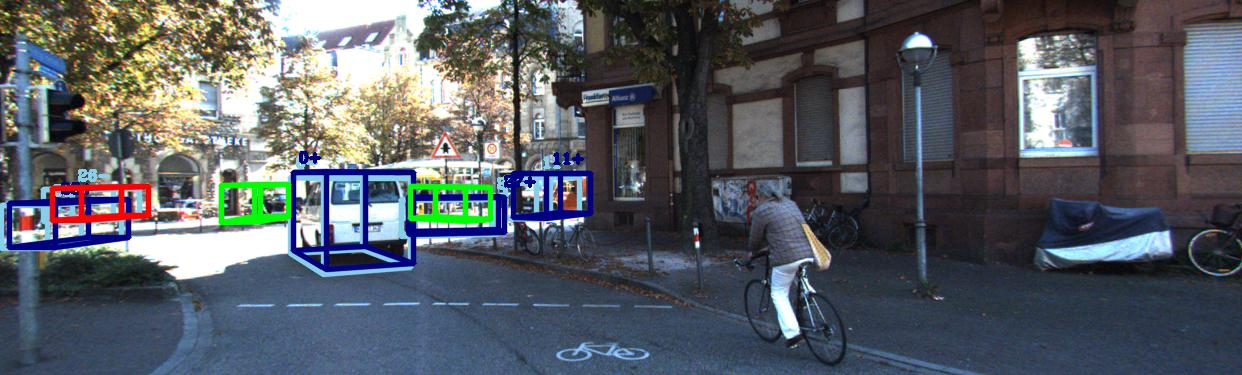
\includegraphics[width=0.85\linewidth]{Q6/23.jpg} }} \\
    \subfloat[frame 024]{{ 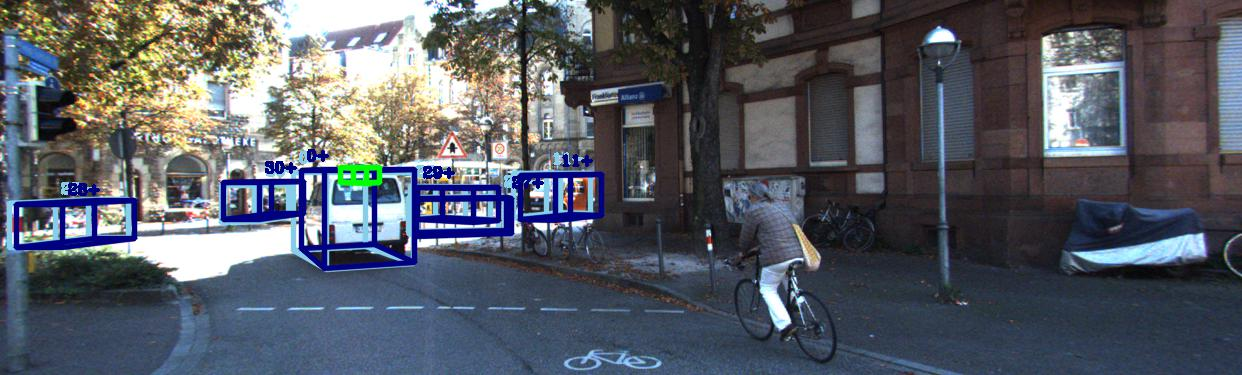
\includegraphics[width=0.85\linewidth]{Q6/24.jpg} }} \\
    \subfloat[frame 025]{{ 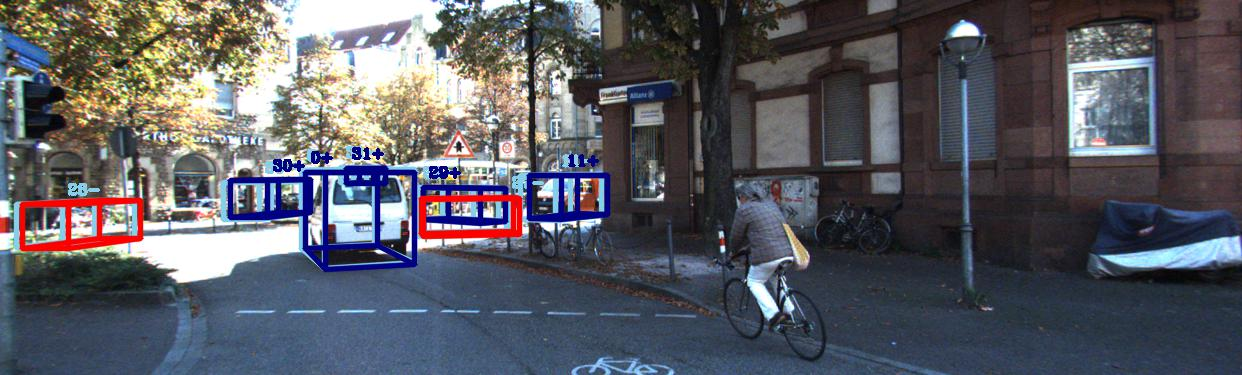
\includegraphics[width=0.85\linewidth]{Q6/25.jpg} }} \\
    \subfloat[frame 026]{{ 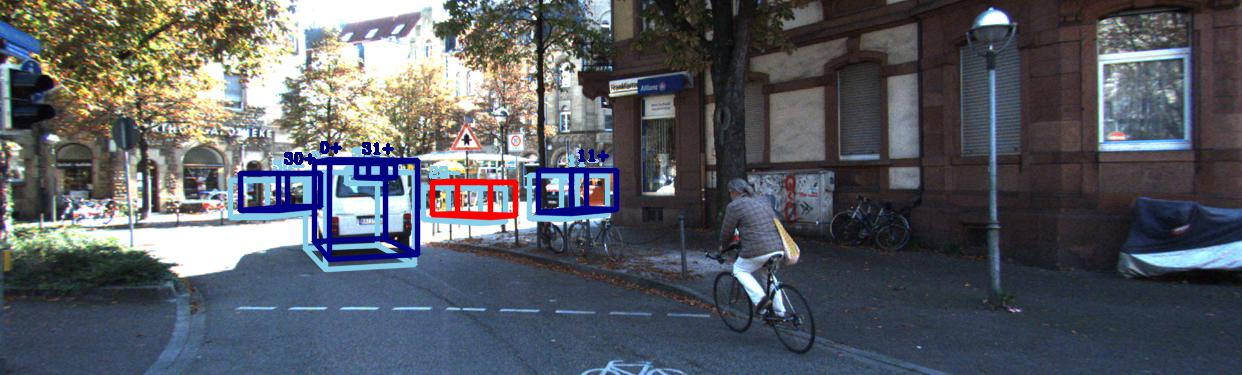
\includegraphics[width=0.85\linewidth]{Q6/26.jpg} }}
    \caption{Tracking results from frame 023 to frame 026 with new trackers (green), old trackers (red), trackers before prediction (skyblue), and trackers after prediction followed by correction (navy).}
    \label{fig:q6-1}
\end{figure}

\begin{figure}[h]
    \centering
    \subfloat[frame 135]{{ 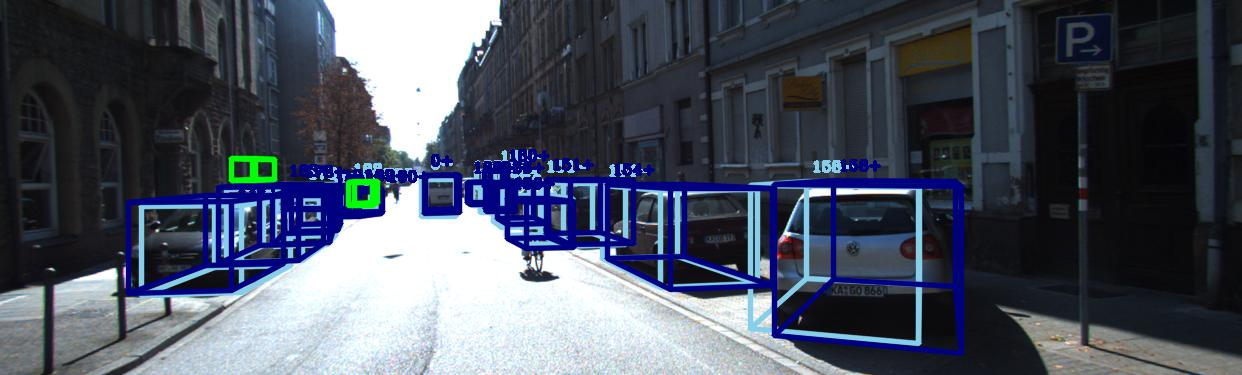
\includegraphics[width=0.85\linewidth]{Q6/135.jpg} }} \\
    \subfloat[frame 136]{{ 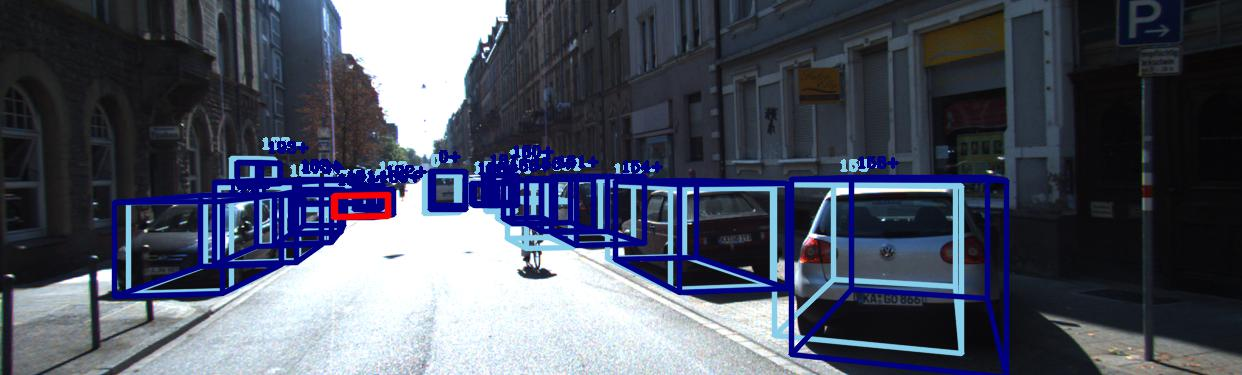
\includegraphics[width=0.85\linewidth]{Q6/136.jpg} }} \\
    \subfloat[frame 137]{{ 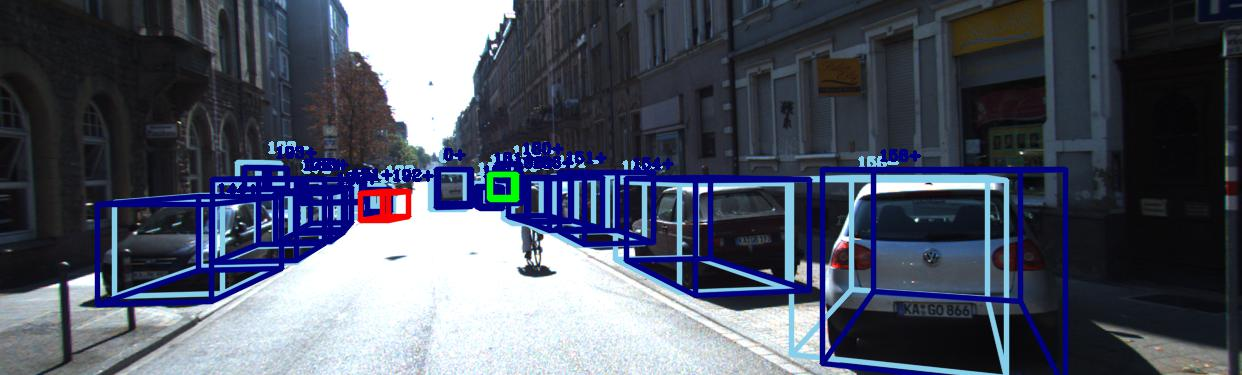
\includegraphics[width=0.85\linewidth]{Q6/137.jpg} }} \\
    \subfloat[frame 138]{{ 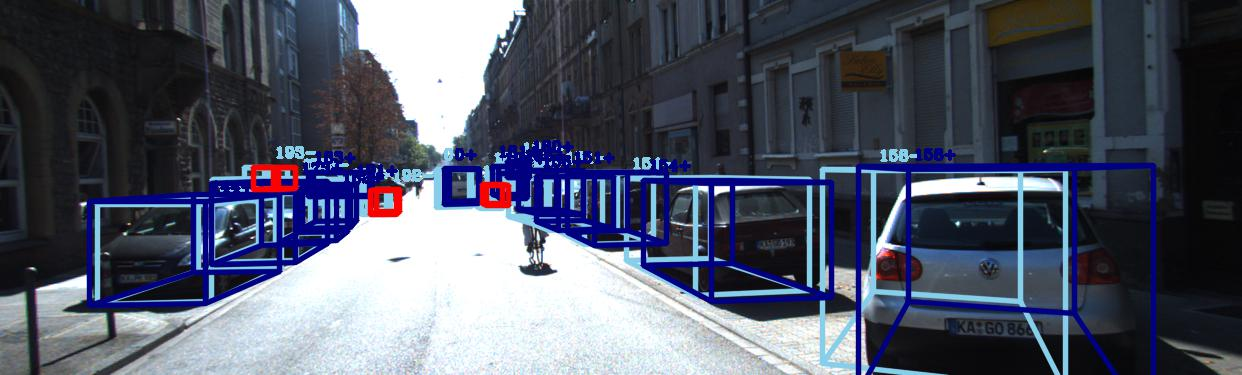
\includegraphics[width=0.85\linewidth]{Q6/138.jpg} }}
    \caption{Tracking results from frame 135 to frame 138 with new trackers (green), old trackers (red), trackers before prediction (skyblue), and trackers after prediction followed by correction (navy).}
    \label{fig:q6-2}
\end{figure}

Other than the generation of new trackers and removal of unused trackers, it is notable that tracker estimations at the beginning (sky blue, with minus signs) in each frame are corrected after its state prediction followed by a measurement update (navy, with minus signs). 

\end{quote}


% DONE
\paragraph{Question 7 (Analysis) [1 pt]:}
Please run the run \texttt{python evaluate.py} and report your MOTA, TPs, ID switches, FRAGs and FPs at the best threshold. Please also visualize at least two failure cases and explain the reason. Please discuss what can be done to avoid these failures.  
\paragraph{Answer:} 
\begin{quote}

Below is the reported metrics of my object detection over 21 sequences at the best threshold:

{\tt \small
=========evaluation with confidence threshold 3.754965 and recall 0.850000========= \\
 sMOTA   MOTA   MOTP    MT     ML     IDS  FRAG    F1   Prec  Recall  FAR     TP    FP    FN     \\
0.9026 0.7672 0.8047 0.7110 0.0691     0   196 0.8974 0.9381 0.8600 0.2018 24497  1616  3987     \\
================================================================================ \\
}

MOTA, TP, ID switches, FRAG, and FP are 0.7672, 24497, 0, 196, and 1616, respectively. 

Here, I analyze two major reasons causing failure in object tracking.
\begin{itemize}
    \item Failure in object detection: If non-objects are detected by the object detection algorithm at a certain frame, all of them are added to new trackers and kept tracked for a while, not until \texttt{time\_since\_update} exceeds \texttt{max\_age}, even though they never indicate `the objects', which is nondesirable.  As a result, they cause `false positive' in object tracking tasks. Fig.~\ref{fig:q7-1} gives an example of how it actually works; in frame 032, several non-objects are detected and started to be tracked, as colored in green. These `false positives' are being kept tracked, not until the death condition (\texttt{time\_since\_update} exceeds \texttt{max\_age}) satisfies at frame 035. 
    \item Mismatching between tracked bounding boxes and detected objects: Another situation may be considered to be a failure in tracking, even if we assume that the object detection algorithm always detects objects properly. This may happen when (1) the tracked bounding boxes are not detected in the new frames or (2) the tracked bounding boxes and the detected objects do not overlap so much, and hence considered to be ``mismatch''. For our case, this is likely to happen for objects far from camera due to the imperfection of our motion model under constant linear velocity assumption, as this assumption leads the tracked bounding boxes deviates from their proper position after prediction stage. To be specific, it becomes problematic when we match small tracked bounding boxes (after prediction) to their detection results, as they appear tiny, are susceptible to even a slight deviation, and may break the matching condition using the IoU threshold easily. As a result, they may cause `false negative' in object tracking missions. Fig.~\ref{fig:q7-2} shows how it actually happens; in frame 141, three different objects are added to trackers---undeniably, they are `correct' objects indicating parked cars. Unfortunately, all of them diminish at frame 144 as no matching between these trackers and the object detection occurs until they meet the death condition (\texttt{time\_since\_update} exceeds \texttt{max\_age}).
\end{itemize}

To avoid such failure, I suggest two key improvements can be made:
\begin{itemize}
    \item Use a better object detection algorithm: This will resolve both cases mentioned above, and it would be the reason why a lot of effort has been made in the domain of object detection.
    \item Use a better motion model: This will contribute to resolving the second issue above, but it is important to keep in mind that there exists a tradeoff between the concreteness and complexity of the motion model. For instance, if we adopt to use a more sophisticated motion model, such as the constant linear acceleration assumption, it leads us to add three other terms (3D linear acceleration) into the state vector and hence the task becomes complicated overall.
\end{itemize}

% examples for tracking failure - case 1: false detections (which usually happens for near objects)
\begin{figure}[h]
    \centering
    \subfloat[frame 032]{{ 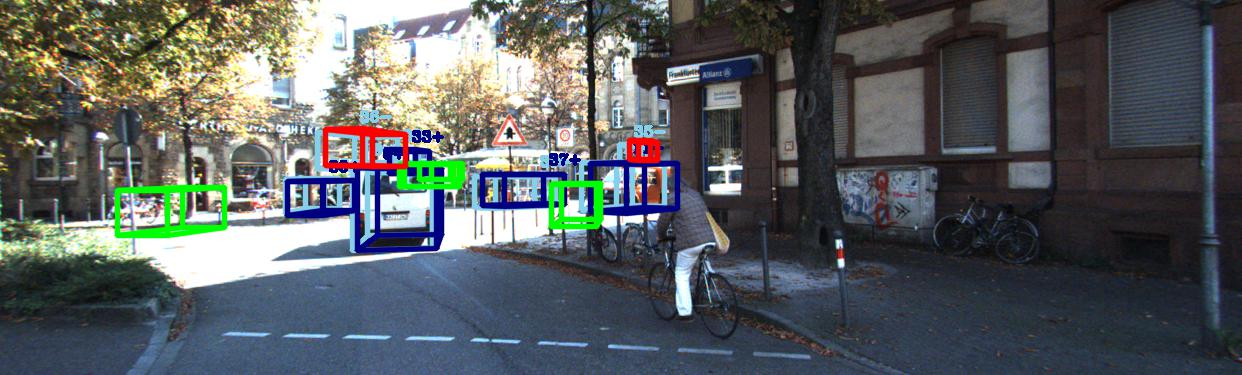
\includegraphics[width=0.85\linewidth]{Q7/32.jpg} }} \\
    \subfloat[frame 033]{{ 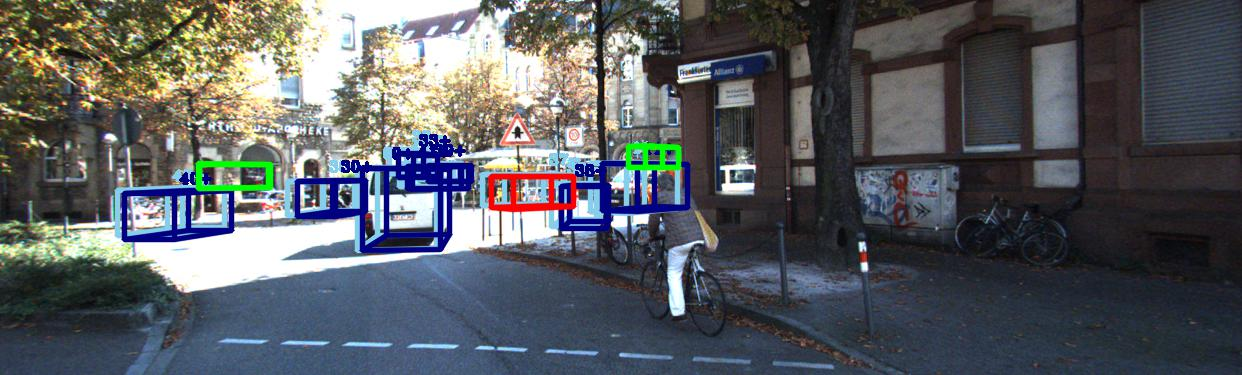
\includegraphics[width=0.85\linewidth]{Q7/33.jpg} }} \\
    \subfloat[frame 034]{{ 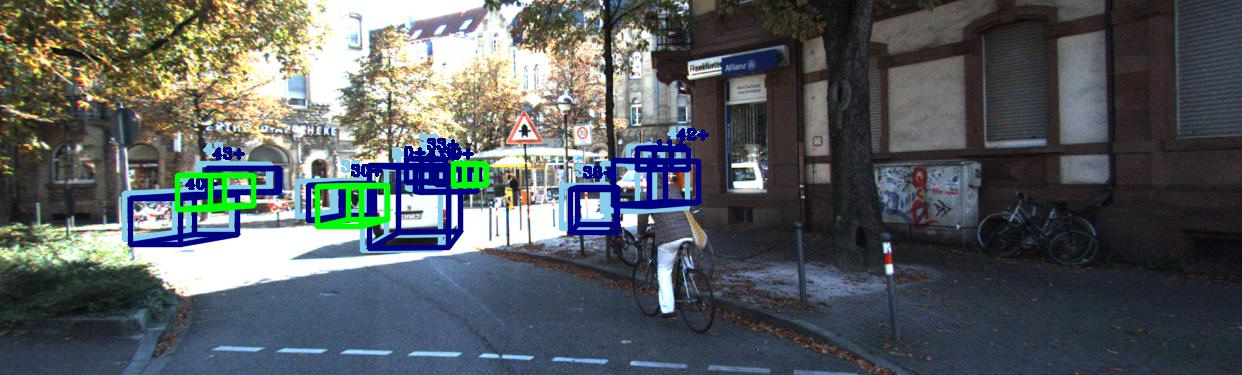
\includegraphics[width=0.85\linewidth]{Q7/34.jpg} }} \\
    \subfloat[frame 035]{{ 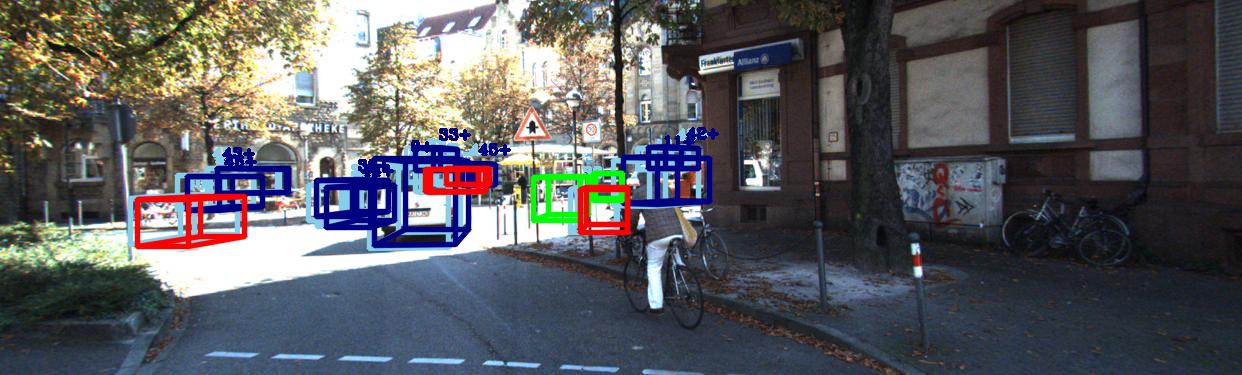
\includegraphics[width=0.85\linewidth]{Q7/35.jpg} }}
    \caption{Examples for tracking failures: tracking results from frame 032 to frame 035.}
    \label{fig:q7-1}
\end{figure}

% examples for tracking failure - case 2: mismatch between trackers and detections (which usually happens for far objects)
\begin{figure}[h]
    \centering
    \subfloat[frame 141]{{ 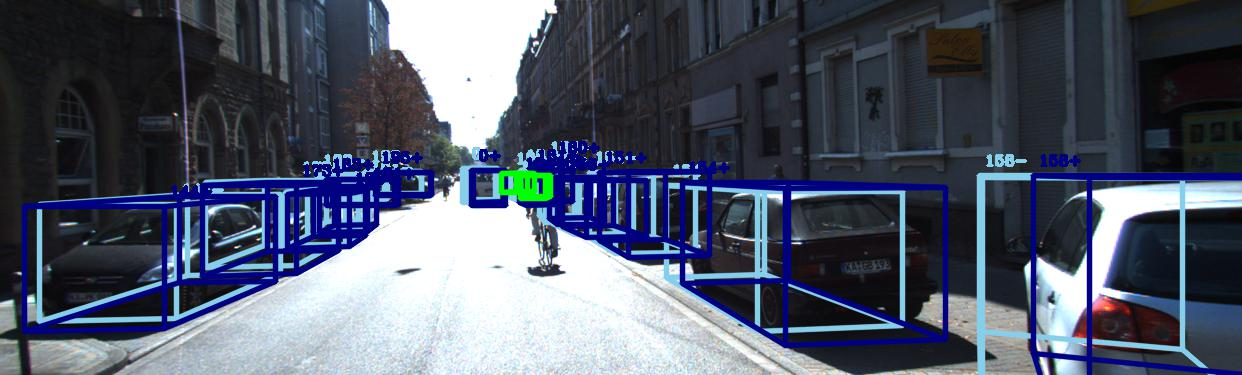
\includegraphics[width=0.85\linewidth]{Q7/141.jpg} }} \\
    \subfloat[frame 142]{{ 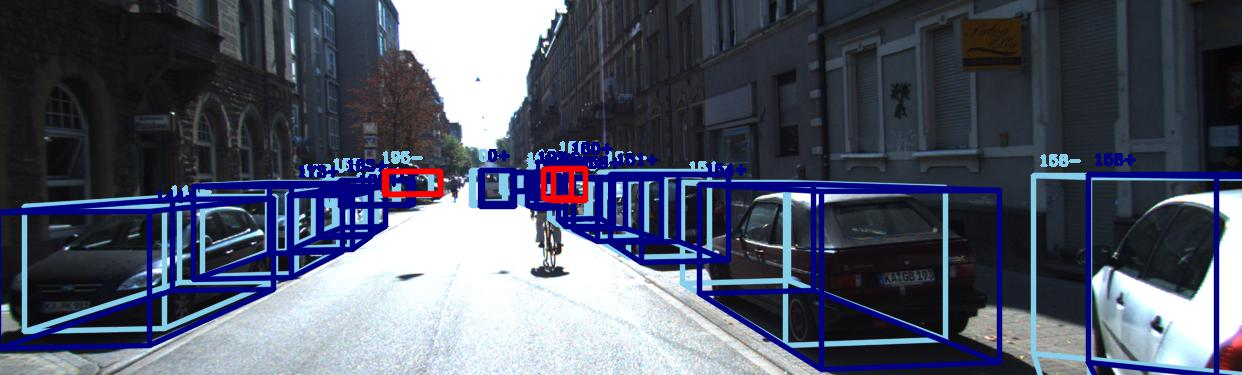
\includegraphics[width=0.85\linewidth]{Q7/142.jpg} }} \\
    \subfloat[frame 143]{{ 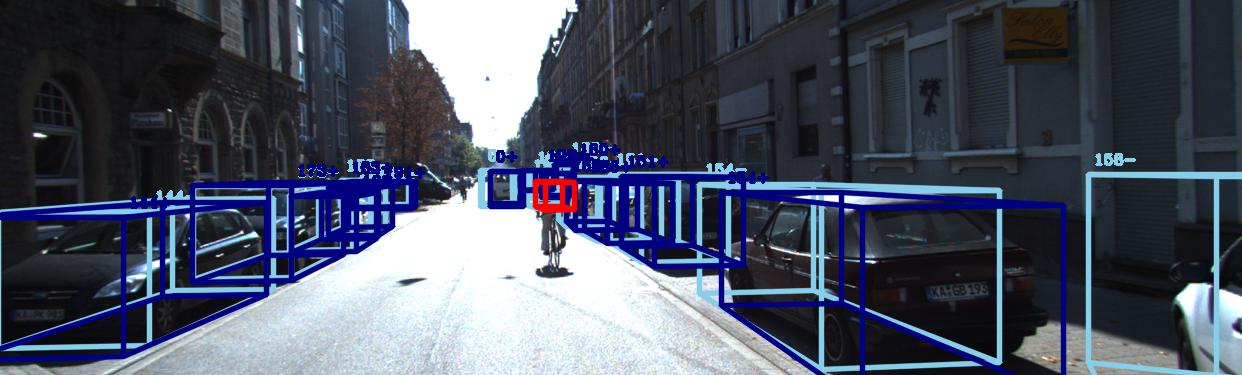
\includegraphics[width=0.85\linewidth]{Q7/143.jpg} }} \\
    \subfloat[frame 144]{{ 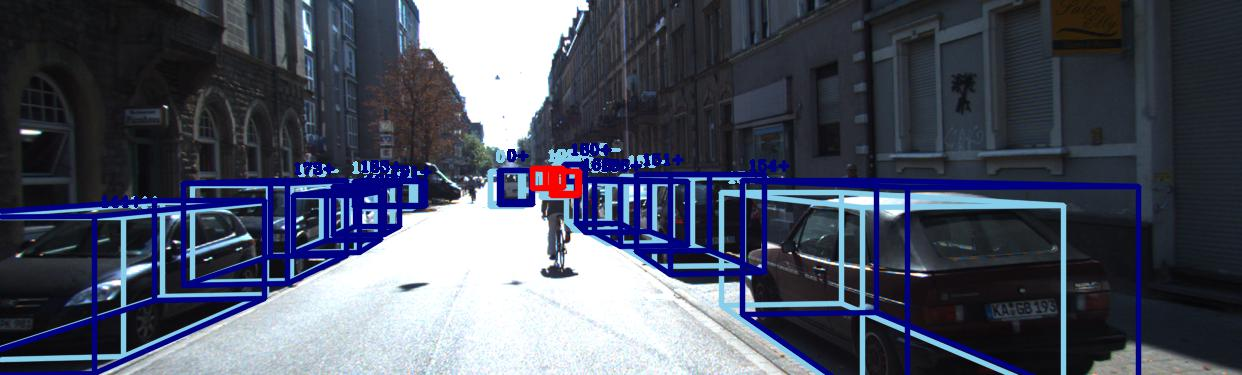
\includegraphics[width=0.85\linewidth]{Q7/144.jpg} }}
    \caption{Examples for tracking failures: tracking results from frame 141 to frame 144.}
    \label{fig:q7-2}
\end{figure}

\end{quote}

\paragraph{Bonus Question (Option 1: Better Matching) [3 pt Bonus]:}
Improve your matching algorithm from greedy to the Hungarian algorithm. You must implement it yourself. Alternatively improve your matching by training a neural network to perform matching based on more than just spatial proximity. Report the tracking performance and compare it against the IOU-based greedy matching through both qualitative and quantitative results. Do you see a performance improvement? Discuss the comparison study results.

\paragraph{Bonus Question (Option 2:Better Dynamics) [3 pt Bonus]:}
Make your kalman filter into an extended kalman filter and implement a bycicle model for dynamics instead of linear. \url{https://www.coursera.org/lecture/intro-self-driving-cars/lesson-2-the-kinematic-bicycle-model-Bi8yE}. 
Report the tracking performance and compare it against linear velocity model through both qualitative and quantitative results. Do you see a performance improvement?  Discuss the comparison study results.

\end{document}. 

\grid
\grid